% \input{\pSections "slide-ftolathm"}
\begin{frame}\frametitle{\ftolathm}
	%
\def\mylambda{3.75}
\def\mymid{\mylambda / 2}
\def\vertspace{0.6}
\def\pttop{(0, \mylambda)}
\def\ptright{(\mylambda, 0)}
%
\newcommand{ \axisblueRow }[0]	{\draw[line width=1.25pt,blue,->,>=stealth]	(-0.1,0) -- \ptright	node[above left=0cm and 0cm of \ptright]{$\bornga{*}$};}
\newcommand{ \axisredRow }[0]	{\draw[line width=1.25pt,red, ->,>=stealth]	(0,-0.1) -- \pttop	node[below right=0cm and 0cm of \pttop]{$\rnlla{}$};}
%
\newcommand{ \axisblueCol }[0]	{\draw[line width=1.25pt,blue,->,>=stealth]	(-0.1,0) -- \ptright	node[above left=0cm and 0cm of \ptright]{$\bornga{}$};}
\newcommand{ \axisredCol }[0]	{\draw[line width=1.25pt,red, ->,>=stealth]	(0,-0.1) -- \pttop	node[below right=0cm and 0cm of \pttop]{$\rnlla{*}$};}
%
\begin{table}[htp]
{\scriptsize{
	\begin{center}
		\begin{tabular}{cccc}
				%
			\multicolumn{4}{c}{\bf{The \ftolathm\ }} \\[5pt]
				%
			& $\A{} \in \mathbb{C}^{^{m \times n}}$ \\%\cline{2-2}
				%
			% ROW SPACE
			\begin{tikzpicture}
				\perps{1/4}
				\node[] at ( \mymid,  \mymid + \vertspace )	{\dg{$ \mat{ccc}{a_{11} & \cdots & a_{1n} }$} };
				\node[] at ( \mymid,  \mymid )				{\dg{$ \vdots$}} ;
				\node[] at ( \mymid,  \mymid - \vertspace )		{\dg{$ \mat{ccc}{a_{m1} & \cdots & a_{mn} }$}} ;
				\axisredRow{}
				\axisblueRow{}
			\end{tikzpicture} &
				%
			% MAPPINGS
			\raisebox{1.5cm}{
			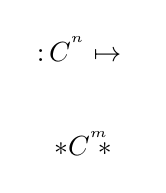
\begin{tikzpicture}
				\node () at (\mymid, \mymid + \vertspace) {$\A{} \colon \mathbb{C}^{^{n}} \mapsto \bornga{}$};
				\node () at (\mymid, \mymid - \vertspace) {$ \bornga{*} \mapsfrom \mathbb{C}^{^{m}} \hspace{-1.5mm} \cocolon \A{*} $};
			\end{tikzpicture} } &&
				%
			% COLUMN SPACE
			\begin{tikzpicture}
				\perps{1/4}
				\node[] at ( \mymid,  \mymid )	{ \dg{ $\mat{c}{a_{11} \\ \vdots \\ a_{m1} } \ \cdots \ \mat{c}{a_{1n} \\ \vdots \\ a_{mn} }$ } };
				\axisredCol{}
				\axisblueCol{}
			\end{tikzpicture} \\[1pt]
				%
				%
			Solution Space & && Data Space \\[1pt]
				%
			$\mathbb{C}^{^{n}} = \codecomprow{*}$ &&& $\mathbb{C}^{^{m}} = \codecompcol{*} $ \\
				%
		\end{tabular}
	\end{center}
	}}
%\caption{A geometric view of the \ftola \ showing the four fundamental subspaces induced by a matrix and the mappings between those subspaces.}
\label{tab:ftola-master}
\end{table}
	%
\end{frame}

\endinput  %  ==  ==  ==  ==  ==  ==  ==  ==  ==
